\documentclass[landscape, 8pt]{extarticle}
\usepackage{geometry}

% \usepackage{showframe}
% \setlength{\fboxsep}{-\fboxrule}

\usepackage[dvipsnames]{xcolor}

\usepackage{adjustbox}

\colorlet{colour1}{Red}
\colorlet{colour2}{Green}
\colorlet{colour3}{Cerulean}

\geometry{
    a4paper, 
    margin=0.17in
}

\pretolerance=0
\hyphenpenalty=0

\usepackage{lmodern}

\usepackage[fontsize=7pt]{scrextend}

\usepackage{multirow}
\usepackage{array}
\usepackage{graphicx} % Required for inserting images
\usepackage{amsmath}
\usepackage{amsfonts}
\usepackage{amsthm}
\usepackage{amssymb}
% \usepackage{preamble}
\usepackage{enumitem}
\setlist{itemsep=0pt}


\usepackage{multicol}
\usepackage{lipsum}
\usepackage[framemethod=TikZ]{mdframed}
% \usepackage{../thmboxes_white}
\usepackage{../thmboxes_v2}
\usepackage{../customs}
\usepackage{float}
% \usepackage{setspace}
\usepackage[nodisplayskipstretch]{setspace}


\newcommand\Tstrut{\rule{0pt}{2.6ex}}       % top strut
\newcommand\Bstrut{\rule[-1.1ex]{0pt}{0pt}} % bottom strut


\setlength{\parskip}{0.2em}

% Custom Definitions of operators
% \DeclareMathOperator{\im}{im}
% \DeclareMathOperator{\Fix}{Fix}
% \DeclareMathOperator{\Orb}{Orb}
% \DeclareMathOperator{\Stab}{Stab}
% \DeclareMathOperator{\send}{send}
% \DeclareMathOperator{\dom}{dom}
% \DeclareMathOperator{\Maps}{Maps}
% \DeclareMathOperator{\sgn}{sgn}
% \DeclareMathOperator{\Mat}{Mat}
% \DeclareMathOperator{\scale}{sc}
% \DeclareMathOperator{\Hom}{Hom}
% \DeclareMathOperator{\id}{id}
% \DeclareMathOperator{\rk}{rk}
% \DeclareMathOperator{\Tr}{tr}
% \DeclareMathOperator{\diag}{diag}
% \DeclareMathOperator{\can}{can}

\usepackage{hyperref} % note: this is the final package

\parindent = 0pt

\renewcommand\labelitemi{\tiny$\bullet$}

\begin{document}

\setlength{\abovedisplayskip}{3.5pt}
\setlength{\belowdisplayskip}{3.5pt}
\setlength{\abovedisplayshortskip}{3.5pt}
\setlength{\belowdisplayshortskip}{3.5pt}

\begin{multicols}{3}
\raggedcolumns


\section*{\huge Metric Spaces Exam Notes}
Made by Leon :) \textit{Note: Any reference numbers are to the lecture notes}

\vspace{-5pt}
\section{Introduction to Metric Spaces}

\begin{dfn}[Definition of a Metric]{def:metric}{1}
    \vspace{-5pt}
    Let $X$ be a non-empty set. A function $d: X \times X \to \mathbb{R} $ is called a \textbf{metric} iff for all $x,\,y,\,z\in X$,
    \vspace{-3pt}
    \begin{itemize}
        \item $d(x,y)\ge 0$ and $d(x,y)=0 \iff x = y$
        \item $d(x,y)=d(y,x)$
        \item $d(x,y)\le d(x,z)+d(z,y)$ (Triangle Inequality)
    \end{itemize}
    \vspace{-5pt}
    A non-empty set $X$ equipped with a metric $d$ is a \textbf{metric space}
\end{dfn}

\vspace{-5pt}
\begin{dfn}[Real Vector Spaces]{dfn:modules-and-vector-spaces}{A}
    \vspace{-5pt}
    A \textbf{real vector space $V$} is a set with two operations $(X, +, \cdot)$, where:
    \vspace{-15pt}
    \begin{itemize}[leftmargin=*]
        \item $+$ is addition, and $\cdot$ is scalar multiplication
        \item $(X, +)$ is an abelian group - i.e. for all (vectors) $x,y,z\in X$:
            \vspace{-5pt}
            \begin{itemize}
                \item \textbf{Closure}: $x + y\in X$
                \item \textbf{Commutativity}: $x + y = y + x$
                \item \textbf{Associativity}: $x + (y + z) = (x + y) + z$
                \item \textbf{Identity}: $\exists 0\in X$ s.t. for all $x\in X$ we have $0 + x = x + 0 = x$
                \item \textbf{Inverse}: $\forall x\in X$ we have $-x$ s.t. $x + (-x) = (-x) + x = 0$
            \end{itemize}
            
            \vspace{-5pt}
            \item Vector space axioms: for all $x,y,z\in X$ and $\mu, \lambda \in \mathbb{R}$ we have:
                \vspace{-5pt}
                \begin{itemize}
                    \item \textbf{Closure-ish thing}: $\lambda x\in X$
                    \item \textbf{Distributivity 1}: $\lambda(x + y) = \lambda x + \lambda y$
                    \item \textbf{Distributivity 2}:$(\lambda + \mu)x = \lambda y + \mu x$
                    \item \textbf{Associativity}: $\lambda (\mu x) = (\lambda \mu) x$
                    \item \textbf{Identity}: $1x = x$
                \end{itemize}
    \end{itemize}
\end{dfn}

\vspace{-5pt}
\begin{dfn}[Normed and Inner Product Spaces]{def:normed-space-inner-space}{B}
    \vspace{-5pt}
    \textrule{\textbf{Def 5 (Normed Vector Spaces)}}

    \vspace{-3pt}
    A \textbf{normed vector space} is a real vector space $X$ equipped with a \textbf{norm}, i.e. a function that assigns to every vector $x\in X$ a real number $\lVert x \rVert$ so that, for all vectors $x$ and $y$ in $X$ and all real scalars $a$:

    \vspace{-5pt}
    \begin{itemize}
        \item $\lVert x\rVert\ge 0 $ and $\lVert x \rVert = 0 \iff x = 0$
        \item $\lVert ax \rVert = \lvert a \rvert\lVert x \rVert$
        \item $\lVert x+y \rVert\le \lVert x \rVert + \lVert y \rVert$
    \end{itemize}

    \vspace{-7pt}
    \longrule{0.08ex}
    \textbf{Remark}: If $(X, \lVert \cdot \rVert)$ is a normed vector space then
    \[d(x,y) = \lVert x - y \rVert\]
    defines a metric in $X$

    % \textbf{Remark}: This is a generalisation of the "length of a vector"


    \textrule{\textbf{Def 6 (Inner Product Spaces)}}

    Let $X$ be a real vector space. An \textbf{inner product} on $X$ is a function that assigns to every pair $(x,y)\in X \times X $ a real number denoted by $\langle x,y \rangle$ and has the following properties:
    \vspace{-3pt}
    \begin{itemize}
        \item $\langle x,x \rangle\ge 0$ and $\langle x,x \rangle = 0 \iff x = 0$
        \item $\langle x,y \rangle = \langle y,x \rangle$
        \item $ax + by, z = a\langle x,z \rangle + b\langle y,z \rangle$
    \end{itemize}

    \vspace{-5pt}
    \longrule{0.08ex}
    A \textbf{real inner product space} is a real vector space equipped with an inner product.
    If $\langle \cdot, \cdot \rangle$ is an inner product on $X$, then
    \vspace{-5pt}
    \begin{itemize}
        \item $\lVert x \rVert = \sqrt{\langle x,x \rangle}$ defines a norm in $X$
        \item $d(x,y) = \lVert x - y \rVert$ defines a metric in $X$
    \end{itemize}
    \vspace{-5pt}
    % \textbf{Remark}: This is a generalisation of the dot product
\end{dfn}


\vspace{-5pt}

\begin{dfn}[$n$-dimensional Euclidean space]{def:ndim-euclidean-space}{C}
    \vspace{-5pt}
    Let $X = \mathbb{R}^{n} = \{(x_{1},x_{2},\dots,x_{n}) : x_{1},x_{2},\dots,x_{n}\in\mathbb{R}\}$
    \newline
    For $x = (x_{1},x_{2},\dots,x_{n})$, $y=(y_{1},y_{2},\dots,y_{n})$ in $\mathbb{R}^{n}$, define
    \[\langle x,y \rangle = x_{1}y_{1} + x_{2}y_{2} + \cdots + x_{n}y_{n} \text{ (inner product)}\]
    \[\lVert x \rVert_{2} = \langle x,x \rangle^{1/2} = \sqrt{x^{2}_{1} + x^{2}_{2} + \cdots + c^{2}_{n}}\text{(norm)}\]
\end{dfn}
\vspace{-5pt}

\begin{xmp}[Examples of Metric Spaces]{xmp:metric-spaces}{D}
    \vspace{-5pt}
    Unless stated otherwise let $X = \mathbb{R}^{n}$. The case $X = \mathbb{R}^{2}$ is listed in \textcolor{red}{red}

    \vspace{-6pt}
    \def\arraystretch{1.5}
    \begin{center}
        \begin{tabular}{|c|l|}
        \hline
        \textbf{Name} & \textbf{Norm and Metric} \\
        \hline
        \multirow{2}{*}{Standard} & $X = \mathbb{R}$ and $\lvert x \rvert = \text{Absolute Value}$ \\
        & $d(x, y) = \lvert x - y \rvert$ \\

        \hline
        \multirow{2}{*}{Taxicab} & $\lVert x \rVert_{1} = \textcolor{red}{\lvert x_{1} \rvert + \lvert x_{2} \rvert} + \cdots \lvert x_{n} \rvert$ \\
                                 & $d_{1}(x, y) = \textcolor{red}{\lvert x_{1} - y_{1} \rvert + \lvert x_{2} - y_{2} \rvert} + \cdots + \lvert x_{n} - y_{n} \rvert$ \\
        \hline
        \multirow{2}{*}{Euclidean} & \parbox{20em}{\vspace{2pt}$\lVert x \rVert_{2} = \sqrt{\textcolor{red}{\lvert x_{1} \rvert^{2} + \lvert x_{2} \rvert^{2}} + \cdots \lvert x_{n} \rvert^{2}}$\vspace{2pt}} \\
                                   & $d_{2}(x, y) = \sqrt{\textcolor{red}{( x_{1} \! - \! y_{1} )^{2} \! + \! ( x_{2} \! - \! y_{2} )^{2}} \! + \cdot\!\cdot +  ( x_{n} \! - \! y_{n} )^{2}}$ \\
        \hline
        \multirow{2}{*}{$p$-metric} & \parbox{20em}{\vspace{2pt}$\lVert x \rVert_{p} = \displaystyle \left( \sum_{k = 1}^{n} \lvert x_{k} \rvert^{p}\right)^{1 /p}$\vspace{2pt}} \\
                                    & \parbox{20em}{\vspace{2pt}$d_{p}(x, y) = \displaystyle \left( \sum_{k = 1}^{n} \lvert x_{k} - y_{k} \rvert^{p}\right)^{1 /p}$\vspace{2pt}} \\
        \hline
        \multirow{2}{*}{Chebyshev} & $\lVert x \rVert_{\infty} = \max \{\textcolor{red}{\lvert x_{1} \rvert, \lvert x_{2} \rvert},\dots, \lvert x_{n} \rvert\}$ \\
                                   & $d(x, y) = \max \{\textcolor{red}{\lvert x_{1} - y_{1} \rvert, \lvert x_{2} - y_{2} \rvert},\dots, \lvert x_{n} - y_{n} \rvert\}$ \\

        \hline
        Discrete & \parbox{20em}{\vspace{2pt}$d(x, y) = \begin{cases}
                0 & x = y \\
                1 & x \ne y
        \end{cases}$\vspace{2pt}} \\
        \hline
            Post Office & \parbox{20em}{\vspace{2pt}$d(x, y) = \begin{cases}
                \lVert x \rVert_{2} + \lVert y \rVert_{2} & x = y \\
                1 & x \ne y
            \end{cases}$\vspace{2pt}} \\
        \hline
    \end{tabular}
    \end{center}

    \begin{figure}[H]
        \centering
        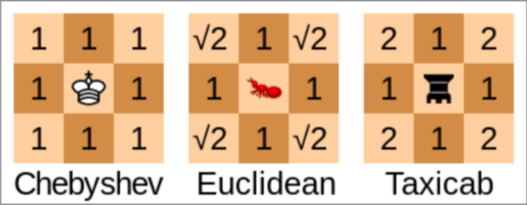
\includegraphics[width=0.8\linewidth]{images/2024-05-14-225838_hyprshot.png}
    \end{figure}

    % TODO: cauchy shwarz?

    % This is the \textbf{Cauchy-Schwarz Inequality}. Various ways to prove this (watch lecture 1)

    \textrule{\textbf{The complex plane}}

    Let $X = \mathbb{C},\, d: \mathbb{C} \times \mathbb{C} \to \mathbb{R} $
    \[d(z,w) = \lvert z - w \rvert\]
    If $z = a+ib, w = c+id,\, a,b,c,d\in\mathbb{R}$, then
    \[z - w = (a - c) + i(b - d)\]
    therefore,
    \[d(z,w) = \sqrt{(a-c)^{2} + (b-d)^{2}}\]

\end{xmp}



\begin{xmp}[Sequence Spaces]{xmp:sequence-spaces}{E}
    \vspace{-5pt}
    \textrule{\textbf{The space $\ell^{1}$}}

    $\ell^{1}$ is the set of real sequences $(x_{n})_{n\in\mathbb{N}}$ where $\sum_{n = 1}^{\infty}\lvert x_{n} \rvert$ converges.

    For $x = (x_{1},\dots,x_{n},\dots)\in \ell^{1}$, $y = (y_{1},\dots,y_{n},\dots)\in \ell^{1}$ we define
    \vspace{-2pt}
    \begin{itemize}[leftmargin=*]
        \item \textbf{Norm}: $\lVert x \rVert_{1} = \sum_{n = 1}^{\infty} \lvert x_{n} \rvert$
        \item \textbf{Metric}: $d_{1}(x, y) = \lVert x - y \rVert_{1} = \sum_{n = 1}^{\infty} \lvert x_{n} - y_{n} \rvert$
    \end{itemize}
        
    \vspace{-2pt}
    \textrule{\textbf{The space $\ell^{2}$}}

    $\ell^{2}$ is the set of real seqs $(x_{n})_{n\in N}$ where $\sum_{n = 1}^{\infty} \lvert x_{n} \rvert^{2}$ converges

    For $x = (x_{1},\dots,x_{n},\dots)\in \ell^{2}$, $y = (y_{1},\dots,y_{n},\dots)\in \ell^{2}$ we define
    \vspace{-6pt}

    \begin{itemize}[leftmargin=*]
        \item \textbf{Inner product}: $\langle x, y \rangle = \sum_{n = 1}^{\infty} x_{n}y_{n}$
        \item \textbf{Norm}: $\lVert x \rVert_{2} = \left(\sum_{n = 1}^{\infty}\lvert x_{n} \rvert^{2}\right)^{1 /2}$
        \item \textbf{Metric}: $d_{2}(x, y) = \lVert x - y \rVert_{2} = \left(\sum_{n = 1}^{\infty}\lvert x_{n} - y_{n} \rvert^{2}\right)^{1 /2}$
    \end{itemize}

    \vspace{-3pt}
    \textbf{Thm}: $\ell^{2}$ is a real vector space

    \textrule{\textbf{The space $\ell^{\infty}$}}

    $\ell^{\infty}$ is the set of all bounded sequences of real numbers
    For $x = (x_{1},\dots,x_{n},\dots),\,y = (y_{1},\dots,y_{n},\dots)\in \ell^{\infty}$
    \vspace{-3pt}
    \begin{itemize}[leftmargin=*]
        \item \textbf{Norm}: $\lVert x \rVert_{\infty} = \sup \{\lvert x_{1} \rvert,\dots,\lvert x_{n} \rvert,\dots\}$
        \item \textbf{Metric}: $\lVert x - y \rVert_{\infty} = \sup \{\lvert x_{1} - y_{1} \rvert,\dots,\lvert x_{n} - y_{n} \rvert,\dots\}$
    \end{itemize}

    \vspace{-3pt}
    \textrule{\textbf{The space $C([a, b])$}}

    $X = C([a, b])$ is the set of all continuous functions $f : [a, b]\to \mathbb{R}$
    \vspace{-3pt}
    \begin{itemize}[leftmargin=*]
        \item \textbf{Norm}: $\lVert f \rVert_{\infty} = \max \{ \lvert f(x) \rvert : a \le x \le b\}$
        \item \textbf{Metric}: $d_{\infty}(f, g) = \lVert f - g \rVert = \max \{\lvert f(x) - g(x) \rvert : a \le x \le b\}$
    \end{itemize}

    \vspace{-3pt}
    \textrule{\textbf{The $L^{1}$ metric}}

    $X$ is the set of all continuous functions $f : [a, b] \to \mathbb{R}$
    \vspace{-3pt}
    \begin{itemize}
        \item \textbf{Norm}: $\lVert f \rVert_{1} = \int_{a}^{b} \lvert f(x) \rvert dx$
        \item \textbf{Metric}: $d_{2}(f, g) = \lVert f - g \rVert_{1} = \int_{a}^{b} \lvert f(x) - g(x) \rvert dx$
    \end{itemize}
    \vspace{-3pt}

    \textrule{\textbf{The $L^{2}$ metric}}

    $X$ is the set of all continuous functions $f : [a, b] \to \mathbb{R}$
    \vspace{-3pt}
    \begin{itemize}
        \item \textbf{Inner Product}: $\langle f, g \rangle = \int_{a}^{b} f(x)g(x) dx$
        \item \textbf{Norm}: $\lVert f \rVert_{2} = \langle f, f \rangle^{1 /2} = \left(\int_{a}^{b} \lvert f(x) \rvert^{2} dx\right)^{1 /2}$
        \item \textbf{Metric}: $d_{1}(f, g) = \left(\int_{a}^{b} \lvert f(x) - g(x) \rvert^{2} dx\right)^{1 /2}$
    \end{itemize}
\end{xmp}

\begin{dfn}[Metric Subspaces]{dfn:metric-subspace}{F}
    \textbf{Ex 7}: Let $(X, d)$ be a metric space and $Y$ a non-empty subset of $X$. Define
    \begin{itemize}
        \item $d_{Y} : Y \times Y \to \mathbb{R}$
        \item $d_{y}(y, y') = d(y, y')$
    \end{itemize}

    Then $d_{Y}$ is a metric on $Y$. $d_{Y}$ is called the \textbf{induced} or \textbf{inherited} metric, and $(Y, d_{Y})$ is said to be a metric subspace of the metric space $(X, d)$
\end{dfn}

\newpage

\begin{thm}[a lack of equality or fair treatment in t...]{dfn:p-metric}{G}
    \textrule{\textbf{Good old fashioned Triangle Inequality}}

    If it ain't broke...
    \[\lvert x + y \rvert \le \lvert x \rvert + \lvert y \rvert \quad \lvert x - y \rvert \ge \big\lvert \lvert x \rvert - \lvert y \rvert \big\rvert \quad \lvert x - y \rvert \le \lvert x - z \rvert + \lvert z - y \rvert\]

    \textrule{\textbf{Cauchy-Schwarz Inequality}}

    For all $x$ and $y$ of an inner product space:
    \[\lvert \langle x, y \rangle \rvert \le \lVert x \rVert \lVert y \rVert\]

    \textrule{\textbf{Minkowski's Inequality}}

    Let $p \ge 1$, and real numbers $x_{i}, y_{i},\,(i = 1,\dots,n)$. Then
    \begin{align*}
        \lVert x + y \rVert_{p} &\le \lVert x \rVert_{p} + \lVert y \rVert_{p} \\
        \left(\sum_{i = 1}^{n} \lvert x_{i} + y_{i} \rvert^{p}\right)^{\frac{1}{p}} &\le \left(\sum_{i = 1}^{n} \lvert x_{i} \rvert^{p}\right)^{\frac{1}{p}} + \left(\sum_{i = 1}^{n} \lvert y_{i} \rvert^{p}\right)^{\frac{1}{p}}
    \end{align*}

    \textrule{\textbf{Ex 56 (Young's Inequality)}}
    
    Let $1 \le p, q \le \infty$ s.t. $\frac{1}{p} + \frac{1}{q} = 1$, and $a, b\le 0$. Then
    \[ab \le \frac{a^{p}}{p} + \frac{b^{q}}{q}\]

    \textrule{\textbf{Thm 169 (Hölder Inequality)}}

    Let $1 \le p, q \le \infty$ s.t. $\frac{1}{p} + \frac{1}{q} = 1$ and $x, y\in \mathbb{R}^{n}$. Then
    \[\sum_{i = 1}^{n} \lvert x_{i}y_{i} \rvert \le \lVert x \rVert_{p} \lVert y \rVert_{q}\]

\end{thm}


\begin{dfn}[Equivalent Norms]{dfn:equivalent-norms}{166}
    \vspace{-5pt}
    Two norms on the same real vector space are said to be equivalent iff their corresponding metrics are equivalent

    \longrule{0.08ex}
    \textbf{Thm 167}: If $\lVert \cdot \rVert_{1}$ and $\lVert \cdot \rVert_{2}$ are norms on the same real vector space $X$ and there exist positive constants $C$ and $C'$ s.t., for all $x\in X$,
    \[D \lVert x \rVert_{1} \le \lVert x \rVert_{2} \le C' \lVert x \rVert_{1}\]
    then they are equivalent


    \textrule{\textbf{Equivalence Theorems of $p$-metrics}}

    \vspace{-10pt}
    \begin{itemize}
        \item[\textbf{171}:] Any of the following norms are equivalent:
            \begin{align*}
                \lVert x \rVert_{p} &= (\lvert x_{1} \rvert^{p} + \cdots + \lvert x_{n} \rvert^{p})^{1 /p},\,x\in \mathbb{R}^{n},\, 1\le p < \infty\\
                \lVert x \rVert_{\infty} &= \max \{\lvert x_{1} \rvert,\dots,\lvert x_{n} \rvert\},\,x\in\mathbb{R}^{n}
            \end{align*}
        \item[\textbf{172}:] Let $1 \le p \le q < \infty$. For all $x\in\mathbb{R}^{n}$:
            \[\lVert x \rVert_{q} \le \lVert x \rVert_{p}\]
            As a consequence,
            \[\lVert x \rVert_{\infty} \le \lVert x \rVert_{q} \le \lVert x \rVert_{p} \le \lVert x \rVert_{1}\]
        \item[\textbf{173}:] All norms in $\mathbb{R}^{n}$ are equivalent

    \end{itemize}
\end{dfn}

\setcounter{subsection}{1}

\begin{dfn}[Open Ball]{def:open-ball}{8}
    Let $(X, d)$ be a metric space, $c$ be a point in $X$, and $r > 0$. The \textbf{open ball} with center $c$ and radius $r$ is defined by
    \[B(c,r) = \{x\in X: d(c,x) < r\}\]
\end{dfn}

% TODO: open ball examples?

% \textbf{Example:} on the real line with the standard metric
% \[b(c,r) = \{x\in\mathbb{R} : \lvert x - c \rvert < r\} = (c - r, c + r)\]
%
% \textbf{Example:} on the real plane with the Euclidean metric, $X = \mathbb{R}^{2}$m
% \[d_{2}(x,y) = \sqrt{\lvert x_{1} - y_{1} \rvert^{2} + \lvert x_{2} - y_{2} \rvert}^{2}\]
% $B(c,r)$ is the open disc with center $c$ and radius $r$
%
% % \longrule{0.08ex}
%
% Watch lecture recording for examples of open balls on:
% \begin{itemize}
%     \item Discrete metric
%     \item $\mathbb{R}^{2}$ with the $d_{1}$ metric
%     \item $\mathbb{R}^{2}$ with the $d_{\infty}$ metric
% \end{itemize}
%

\section{Convergence}

% On the real line, $x_{n}\to x$ iff for every positive $\epsilon$, there exists an index $N$ such that for all indices $n$ where $n\ge N$, we have $\lvert x_{n} - x \rvert < \epsilon$.

\begin{dfn}[Convergent Sequence]{metric-convergence}{15}
    Let $(X,d)$ be a metric space, $(x_{n})^{\infty}_{n=1}$ be a sequence in $X$, and $x\in X$. We say that $(x_{n})^{\infty}_{n=1}$ converges to $x$ iff for every $\epsilon > 0$, there exists an index $N$ s.t. for all $n\ge N$ we have $d(x_{n}, x) < \epsilon$.

    Observe that:
    \vspace{-5pt}
    \begin{itemize}
        \item $d(x_{n}, x)< \epsilon$ is equivalent to $x_{n}\in B(x,\epsilon)$.
        \item $x_{n}\to x$ in $(X,d)$ iff $d(x_{n}, x)\to 0$ on the real line
    \end{itemize}
\end{dfn}

\begin{thm}[Uniqueness of metric limit]{thm:uniqueness-metric-limit}{16}
    \begin{itemize}
        \item Let $(X,d)$ be a metric space, and $x,x'\in X,\,x\ne x'$. Then there exists a positive radius $r$ s.t. $B(x,r)\cap B(x',r) = \emptyset$
        \item A sequence in a metric space can have at most one limit
    \end{itemize}
\end{thm}

\begin{dfn}[Bounded Sequence]{def:bounded-sequence}{19}
    A sequence in a metric space is said to be \textbf{bounded} iff there exists an open ball that contains all of its terms

    \longrule{0.08ex}
    \textbf{Note}: this is the same definition as ``sequence is bounded if there is upper and lower bound'', as open ball implies the same thing

    \longrule{0.08ex}
    \textbf{Thm 20}: Every convergent sequence is bounded
\end{dfn}

\stepcounter{subsection}

\begin{dfn}[Cauchy Sequence]{def:cauchy-seq}{21}
    A sequence $(x_{n})^{\infty}_{n=1}$ in a metric space $(X,d)$ is said to be a \textbf{Cauchy sequence} iff for every positive $\epsilon$, there exists an index $N$, s.t. for all indices $n,m$ with $n,m\ge N$,
    \[d(x_{n}, x_{m}) < \epsilon\]

    \longrule{0.08ex}
    \textbf{Thm 22}: If a sequence in a metric space converges, then it is a Cauchy sequence. \textbf{Note}: the converse is not true
\end{dfn}

\begin{dfn}[Complete Metric Spaces]{def:complete-ms}{24}
    A metric space is said to be \textbf{complete} if and only if every Cauchy Sequence is convergent
\end{dfn}

\begin{xmp}[Examples of Complete Metric Spaces]{xmp:complete-ms}{25}
    \begin{itemize}
        \item $\mathbb{R}$ with the standard metric is complete
        \item $\mathbb{Q}$ with the standard metric is not complete
        \item $(0,1)$ with the standard metric is not complete
        \item $[0,1]$ with the standard metric is complete
        \item $\mathbb{R}^{n},\,\ell^{p},\,C([a,b])$ is complete (proof later)
    \end{itemize} 
\end{xmp}

\begin{dfn}[Open Sets and Closed Sets]{def:open-closed-set}{26}
    \vspace{-5pt}
    Let $(X,d)$ be a metric space.
    \vspace{-5pt}
    \begin{itemize}
        \item A subset $G$ of $X$ is said to be \textbf{open} iff for every point $x$ in $G$ there exists a positive radius $r$ such that $B(x,r)\subseteq G$.
        \item A subset $F$ of $X$ is said to be \textbf{closed} iff $F^{c}$ is open
    \end{itemize}
\end{dfn}

\begin{dfn}[Discrete Spaces and Clopens]{def:discrete-ms}{31}
    \vspace{-5pt}
    A metric space is called \textbf{discrete} iff all its subsets are open (equiv. all subsets are closed)

    \textbf{Example:} $[0,1]\cap (2,3)$

    \longrule{0.08ex}
    \textbf{Def 33}: A set that is both open and closed is called \textbf{clopen}
\end{dfn}

\vspace{-5pt}
\begin{thm}[Properties of open and closed sets]{thm:open-set-props}{34}
    \vspace{-5pt}
    Let $(X,d)$ be a metric space
    \vspace{-5pt}
    \begin{enumerate}
        \item The union of \textbf{any family} of open sets is an open set
        \item The intersection of \textbf{finitely many} open sets is an open set
        \item The intersection of \textbf{any family} of closed sets is an closed set
        \item The union of \textbf{finitely many} closed sets is an closed set
    \end{enumerate}
\end{thm}

\vspace{-5pt}
\begin{rem}[Infinite open sets]{thm:infinite-open-sets}{35}
    \vspace{-5pt}
    The intersection of infinitely many open sets isn't always an open set
    
    e.g., let $G_{n} = (- \frac{1}{n}, \frac{1}{n}), n = 1,2,\dots$ on $\mathbb{R}$ with the standard metric.

    Each $G_{n}$ is open but
    \[\bigcap\limits_{n = 1}^{\infty} G_{n} = \{0\}\]
\end{rem}

\vspace{-5pt}
\begin{thm}[Relatively open sets]{thm:relatively-open}{18}
    \vspace{-5pt}
    Let $(X,d)$ be a metric space and $A$ a nonempty subset of $X$ equipped with the induced metric $d_{A}$. Let $G\subseteq A$. Then $G$ is open in $(A, d_{A})$ iff there exists a subset $O$ of $X$, open in $(X,d)$, s.t. $G = A \cap O$

    The open sets of $(A, d_{A})$ are referred to as \textbf{relatively open}
\end{thm}

\vspace{-5pt}
\begin{thm}[]{thm:open-set-converge}{36}
    \vspace{-5pt}
    Let $(X, d)$ be a metric space, $(x_{n})^{\infty}_{n=1}$ be a sequence in $X$ and $x$ be a point in $X$.

    $x_{n}\to x$ iff every open set that contains $x$ contains eventually all terms of the sequence
\end{thm}

\vspace{-5pt}
\begin{dfn}[Neighbourhoods of points]{def:neighbourhood}{H}
    \vspace{-5pt}
    An \textbf{open neighbourhood} of a point $x$ is any open set that has $x$. 

    $x_{n}\to x$ iff every open neighbourhood of $x$ contains eventually all terms of the sequence.

    \longrule{0.08ex}
    A \textbf{neighbourhood} of a point $x$ is a set that contains an open neighbourhood of $x$.

    $x_{n}\to x$ iff every neighbourhood of $x$ contains eventually all terms of the sequence.
\end{dfn}

\begin{rem}[Infinite closed sets]{thm:infinite-closed-sets}{38}
    \vspace{-5pt}
    The union of infinitely many closed sets is not always a closed set.

    For example, let $F_{n} = [\frac{1}{n}, 1], n=1,2,\dots,$ on the real line with the standard metric.
    Each $F_{n}$ is closed but
    \[\bigcup\limits_{n = 1}^{\infty}F_{n} = (0,1]\]
    is not closed.
\end{rem}

\newpage
\begin{thm}[]{thm:closed-ms-convergence}{41}
    \vspace{-5pt}
    A subset $F$ of a metric space is closed iff the limit of every convergent sequence of elements of $F$ belongs to $F$

    \longrule{0.08ex}
    \vspace{-13pt}
    \begin{itemize}[leftmargin=*]
        \item In any metric space $(X,d)$, singletons $F = \{x\}$ are closed.
        \item In any metric space, any finite set is closed because
            \[\{x_{1},\dots,x_{n}\} = \{x_{1}\}\cup \cdots \cup \{x_{n}\}\]
    \end{itemize}
\end{thm}

\begin{dfn}[Closure]{def:closure}{43}
    \vspace{-5pt}
    Let $(X, d)$ be a metric space and $A \subseteq X$. The \textbf{closure} of $A$, deonted by $\overline{A}$, is the smallest closed subset of $X$ that contains $A$

    There exists at least one closed subset of $X$ that contains $A$, namely $X$ itself. The smallest closed subset of $X$ that contains $A$ is
    \[\bigcap\limits_{\substack{A \subseteq F \subseteq X\\
    F \text{closed}}} F\]
\end{dfn}

\begin{thm}[Properties of Closure]{thm:closure-props}{44}
    \vspace{-5pt}
    Let $(X, d)$ be a metric space and $A,\,B \subseteq X$.
    \vspace{-15pt}
    \begin{multicols}{2}
        \begin{enumerate}[leftmargin=*]
            \item $\overline{\emptyset} = \emptyset$ and $\overline{X} = X$
            \item $A \subseteq \overline{A}$ and $\overline{A}$ is closed
            \item $A$ is closed iff $A = \overline{A}$
            \item $\overline{\overline{A}} = \overline{A}$
            \item If $A \subseteq B$, then $\overline{A} \subseteq \overline{B}$
            \item $\overline{A \cup B} = \overline{A} \cup \overline{B}$
        \end{enumerate}
    \end{multicols}
\end{thm}


\begin{dfn}[Dense Subset of a Metric Space]{def:dense-subset}{49}
    Let $(X, d)$ be a metric space. A subset $D \subseteq X$ is \textbf{dense} iff $\overline{D} = X$

    \longrule{0.08ex}
    \textbf{Random Fact}: In $\mathbb{R}^{n}$ with the Euclidean metric $d_{2}$, $\mathbb{Q}^{n}$ is dense.
\end{dfn}

\begin{thm}[Adherent Points]{thm:closure-equivalence}{50}
    \vspace{-5pt}
    Let $(X, d)$ be a metric space, $A \subseteq X, x\in X$. The following are equiv.
    \vspace{-10pt}
    \begin{enumerate}
        \item $x\in\overline{A}$
        \item For every positive $r$, $B(x,r) \cap A \ne \emptyset$
        \item There exists a sequence $(a_{n})_{n\in \mathbb{N}}$ with $a_{n}\in A$ for all $n$, such that $a_{n}\to x$
    \end{enumerate}
    \vspace{-5pt}
    A point $x$ with any of these properties is called an \textbf{adherent point} of $A$. So, $\overline{A}$ is the set of all adherent points of $A$.
\end{thm}

\begin{dfn}[Limit points of sets]{def:limit-point}{52}
    Let $(X, d)$ be a metric space, $A \subseteq X$ and $x\in X$. We say that $x$ is a \textbf{limit point} or an \textbf{accumulation point} of $A$ iff every open ball centered at $x$ contains an element of $A$ distinct from $x$, i.e.
    \[\forall r > 0 \quad (B(x,r) \backslash \{x\}) \cap A \ne \emptyset\]
    The set of all limit points of $A$ is called the \textbf{derived set} of $A$ and is denoted by $A'$ or $\tilde{A}$.

    \longrule{0.08ex}
    \textbf{Thm 78}: Let $(X, d_{X})$ and $(Y, d_{Y})$ be metric spaces, $x_{0}$ be a limit point of $X$, $y_{0}\in Y$ and $f : X \to Y$ be a function.

    We say that $\lim_{x\to x_{0}} f(x) = y_{0}$ iff for all $\epsilon > 0$, there exists $\delta > 0$ such that for all $x\in B_{X}(x_{0}, \delta) \backslash \{x_{0}\}$ we have
    \[f(x)\in B_{Y}(y_{0}, \epsilon)\]
\end{dfn}

\vspace{-5pt}
\begin{dfn}[Continuity at a point]{def:metric-point-continuity}{54}
    \vspace{-5pt}
    Let $(X, d_{X}),\, (Y,d_{Y})$ be metric spaces and $f: X \to Y $ be a function. We say that $f$ is \textbf{continuous at a point} $x_{0}$ in $X$ iff...
    \vspace{-8pt}

    \begin{itemize}[leftmargin=*]
        \item for every $\epsilon > 0$, there exists a $\delta > 0$, such that, for all $x\in X$ with $d_{X}(x,x_{0}) < \delta$ we have 
            \[d_{Y}(f(x), f(x_{0})) < \epsilon\]
        \item for every $\epsilon > 0$, there exists a $\delta > 0$, such that, for all $x\in B_{X}(x_{0}, \delta)$ we have 
            \[f(x)\in B_{Y}(f(x_{0}), \epsilon)\]
        \item \textbf{Thm 57}: for every open nbhd $G$ of $f(x_{0})$, there exists an open nbhd $O$ of $x_{0}$ such that, for all $x\in O$, we have $f(x) \in G$

    \end{itemize}

    \vspace{-5pt}
    \textrule{\textbf{Def 55 (Continuity of a Function)}}

    Let $(X, d_{X}), (Y, d_{Y})$ be metric spaces. A function $f: X \to Y $ is said to be \textbf{continuous} iff it is continuous at every point in $X$
\end{dfn}

\vspace{-5pt}
\begin{thm}[Continuity and Convergence]{thm:continuity-conv-equivalence}{58}
    \vspace{-5pt}
    Let $(X, d_{X}),\, (Y, d_{Y})$ be metric spaces, $x_{0}$ be a point in $X$, and $f : X \to Y$ be a function. The following are equivalent:
    \vspace{-5pt}
    \begin{enumerate}
        \item $f$ is continuous at $x_{0}$
        \item For every sequence $(x_{n})^{\infty}_{n = 1}$ in $X$, if $x_{n}\xrightarrow[n\to +\infty]{}$ in $(X, d_{X})$, then $f(x_{n}) \xrightarrow[n\to +\infty]{} f(x_{0})$ in $(Y, d_{Y})$
    \end{enumerate}
\end{thm}

\vspace{-5pt}
\begin{thm}[Continuity and Open Sets]{def:continuity-open-sets}{59}
    Let $(X, d_{X}),\,(Y, d_{Y})$ be metric spaces. A function $f: X \to Y $ is continuous iff the inverse image $f^{-1}(G)$ of any open subset $G$ of $Y$ is an open subset of $X$
\end{thm}

\vspace{-5pt}
\begin{dfn}[Topological Space]{def:topological-space}{60}
    \vspace{-5pt}
    A \textbf{topological space} is a set $X$ together with a family $\mathcal{T}$ of subsets of $X$ that has the following properties:
    \vspace{-5pt}
    \begin{itemize}
        \item $\emptyset,X\in \mathcal{T}$
        \item Any union of elements of $\mathcal{T}$ is an element of $\mathcal{T}$
        \item Any finite intersection of elements of $\mathcal{T}$ is an element of $\mathcal{T}$
    \end{itemize}
    \vspace{-5pt}
    $\mathcal{T}$ is called a \textbf{topology} and the elements of $\mathcal{T}$ are called \textbf{open sets}
\end{dfn}

\vspace{-5pt}
\begin{dfn}[Continuity of Topological Spaces]{def:topological-continuity}{61}
    \vspace{-5pt}
    \begin{itemize}[leftmargin=*]
        \item Let $(X, \mathcal{T}_{X})$ and $(Y, \mathcal{T}_{Y})$ be two topological spaces. A function $f : X \to Y$ is said to be \textbf{continuous} iff for every $G$ in $\mathcal{T}_{Y}$ the pre-image $f^{-1}(G)$ is an element of $\mathcal{T}_{X}$.
        \item $f$ is said to be a \textbf{homeomorphism} iff it is a continuous bijection and its inverse is continuous.
        \item If such a homeomorphism exists then $(X, \mathcal{T}_{X})$ and $(Y, \mathcal{T}_{Y})$ are said to be \textbf{homeomorphic}
    \end{itemize}
\end{dfn}

\begin{thm}[$d : X \times X \to \mathbb{R}$ is continuous]{thm:metric-space-continuity}{66}
    \vspace{-5pt}
    Let $(X, d)$ be a metric space. $f: X \times X \to \mathbb{R} $ is continuous, where

    \vspace{-5pt}
    \begin{itemize}
        \item $\mathbb{R}$ is equipped with the standard metric.
        \item $X \times X$ is equipped with the product metric
    \end{itemize}

     
\end{thm}

\begin{dfn}[Bounded Linear Operators]{def:bounded-linear-operators}{67}
    A linear operator $T : X \to Y$ is said to be \textbf{bounded} iff there exists a positive constant $C$ such that, for all $x\in X$,
    \[\lVert T(x) \rVert_{Y} \le C \lVert x \rVert_{X}\]

    \longrule{0.08ex}
    \textbf{Thm 68}: Let $T: X \to Y $ be a linear operator. The following are equivalent:
    \vspace{-13pt}
    \begin{multicols}{3}
    \begin{enumerate}[leftmargin=*]
        \item $T$ is continuous
        \item $T$ is continu. at $0$
        \item $T$ is bounded
    \end{enumerate}
    \end{multicols}
\end{dfn}

\begin{dfn}[Lipschitz Functions]{def:lipschitz-functions}{70}
    Let $(X, d_{X}),\,(Y, d_{Y})$ be metric spaces. A function $f : X \to Y$ is said to be a \textbf{Lipschitz} function iff there exists a constant $L$ such that for all $x,x'\in X$,
    \[d_{Y}(f(x), f(x')) \le L d_{X}(x,x')\]
    If $L < 1$, $f$ is said to be a \textbf{contraction}

    If $f : \mathbb{R} \to \mathbb{R}$ is a Lipschitz function and $x$ is any point in $\mathbb{R}$, then for any $x\in \mathbb{R}$ we have
    \[\lvert f(x) - f(x') \rvert \le L\lvert x - x' \rvert\]
    For $x \ge x'$ this can be expanded to
    \[f(x') - L(x - x') \le f(x) \le f(x') + L(x - x')\]

    \textrule{\textbf{Lipschitz Theorem Bank}}

    \vspace{-8pt}
    \begin{itemize}
        \item[\textbf{71}:] Every Lipschitz function is continuous
        \item[\textbf{175:}] Let $(X, d_{X})$ and $(Y, d_{Y})$ be two metric spaces, and $f : X \to Y$ be a Lipschitz function. Then there exists a smallest Lipschitz constant of $f$ 
        \item[\textbf{176}:] Let $I$ be a non-degenerate open interval on the real line and let $f : I \to \mathbb{R}$ be a differentiable function. Then $f$ is Lipschitz iff $f'$ is bounded. When that is the case,
            \[\lvert f \rvert_{\text{Lip}} = \sup \{\lvert f'(x) \rvert : x\in I\}\]
    \end{itemize}

\end{dfn}

\begin{dfn}[Fixed Points]{def:fixed-points}{72}
    A \textbf{fixed point} of a function $f: S \to S $ where $S$ is a non-empty set, is any element $x$ of $S$ such that $f(x) = x$

    Solving equations can sometimes be reduced to finding fixed points
\end{dfn}

\begin{thm}[Banach's Fixed Point Theorem]{thm:complete-ms-fixed-point}{75}
    Let $(X, d)$ be a complete metric space and let $f : X \to X$ be a contraction. Then $f$ has a unique fixed point
\end{thm}


\begin{dfn}[Equivalent Metrics]{def:equivalent-metrics}{76}
    Two metrics on the same non-empty set $X$ are said to be \textbf{equivalent} iff they have the same open sets

    \longrule{0.08ex}
    \textbf{Thm 77}: Let $d_{1}$ and $d_{2}$ be metrics on the same non-empty set $X$. If there exist positive constants $C$ and $C'$ such that for all $x, y$ in $X$,
    \[Cd_{1}(x, y) \le d_{2}(x, y) \le C'd_{1}(x, y)\]
    then $d_{1}$ and $d_{2}$ are equivalent
\end{dfn}



\newpage

\section{Completeness}
\begin{thm}[Completeness of the Classical Spaces]{thm:completeness-of-classical-spaces}{I}
    \vspace{-5pt}
    Some examples of complete metric spaces:

    \vspace{-6pt}
    \begin{center}
    \def\arraystretch{1.7}
    \begin{tabular}{ |c|c|c|c|c| }
        \hline
        \textbf{79}: $(\mathbb{R}^{n}, d_{2})$ & \textbf{80}: $\ell^{2}$ & \textbf{81}: $\ell^{p}$ & \textbf{82}: $C([a, b])$ & \textbf{83}: $\ell^{\infty}$ \\
        \hline
    \end{tabular}
    \end{center}

    \vspace{-3pt}
    \textrule{\textbf{Exercise 31}}
    \vspace{-8pt}

    \begin{itemize}[leftmargin=*]
        \item Let $(X, d_{X})$ and $(Y, d_{Y})$ be two metric spaces and assume that $(Y, d_{Y})$ is complete.
        \item Let $C(X, Y)$ be the set of all continuous and bounded functions from $X$ to $Y$. For $f, g\in C(X, Y)$ define
            \[D(f, g) = \sup \{d_{Y}(f(x), g(x)) : x\in X\}\]
        \item Then $D$ is a metric and the metric space $(C(X, Y), D)$ is complete
    \end{itemize}
\end{thm}

\vspace{-5pt}
\begin{dfn}[The product space \texorpdfstring{$X^{n}$}{Xn}]{dfn:x-n-product-space}{83}
    \vspace{-5pt}
    Let $(X, d)$ be a metric space and $n\in \mathbb{N}$. Define $D : X^{n} \to \mathbb{R}$ by
    \[D(x_{1}, x_{2}) = d(x_{11}, x_{21}) + d(x_{12}, x_{22}) + \cdots + d(x_{1n}, x_{2n})\]

    \vspace{-5pt}
    \textrule{\textbf{Lemma Bank}}

    \vspace{-8pt}
    \begin{itemize}
        \item[\textbf{Ex.33}:] $D$ is a metric and a sequence converges in $(X^{n}, D)$ iff it \newline converges componentwise
        \item[\textbf{Ex.34}:] If $(X, d)$ is complete then $(X^{n}, D)$ is complete
    \end{itemize}
\end{dfn}

\vspace{-5pt}
\begin{dfn}[The product space \texorpdfstring{$X^{\mathbb{N}}$}{X^N}]{dfn:x-natural-product-space}{84}
    \vspace{-5pt}
    Let $B^{A}$, where $A, B$ are sets, be the set of all functions from $A$ to $B$

    \longrule{0.08ex}
    \textbf{Def 85:} Let $(X, d)$ be a metric space. Define a metric $D : X^{\mathbb{N}} \times X^{\mathbb{N}} \to \mathbb{R}$ by
    \[D(x_{1}, x_{2}) = \sum_{n = 1}^{\infty} \frac{1}{2^{n}} \frac{d(x_{1n}, x_{2n})}{1 + d(x_{1n}, x_{2n})}\]

    \vspace{-8pt}
    \begin{itemize}[leftmargin=*]
        \item $x_{1} = (x_{11},\dots, x_{1n},\dots)$, $x_{2} = (x_{21},\dots,x_{2n},\dots)$
        \item $(X^{\mathbb{N}}, D)$ is called a \textbf{product space}
    \end{itemize}
\end{dfn}

\vspace{-5pt}
\begin{thm}[Product space Convergence \& Completeness]{thm:product-space-convergence}{J}
    \vspace{-5pt}
    \textrule{\textbf{Thm 86 (Convergence)}}

    Let $(X, d)$ be a metric space, let $(x_{k})_{k=1}^{\infty}$ be a sequence in $X^{\mathbb{N}}$ and let $x\in X^{\mathbb{N}}$. Write $x_{k} = (x_{k 1},\dots, x_{kn},\dots)$ and $x = (l_{1},\dots,l_{n},\dots)$. Then, $x_{k} \xrightarrow[k \to +\infty]{(X^{\mathbb{N}}, D)} x$ if and only if, for all $n$, $x_{kn}\xrightarrow[k \to +\infty]{(X^{\mathbb{N}} l_{n}}$

    \textrule{\textbf{Thm 87 (Completeness)}}

    Let $(X, d)$ be a complete metric space. Then the product space $(X^{\mathbb{N}}, D)$ is complete.
\end{thm}

\vspace{-5pt}
\begin{thm}[Completeness of \texorpdfstring{$\mathbb{R}$}{R}]{thm:completeness-of-R}{K}
    \vspace{-5pt}
    \begin{itemize}[leftmargin=*]
        \item \textbf{Thm (Least Upper Bound Principle)}: Every non-empty bounded above subset of $\mathbb{R}$ has a least upper bound
        \item \textbf{Thm 88 (Monotone Convergence)}: Every bounded monotone sequence of real numbers has a limit
        \item \textbf{Thm/Ex. 36 ($\epsilon$-convergence)}: Let $A$ be a non-empty boudned subset of $\mathbb{R}$ and let $\epsilon$ be positive. If the distance between any two elements of $A$ is $< \epsilon$, then
        \[\sup(A) - \inf(A) \le \epsilon\]
        \vspace{-13pt}
        \item \textbf{Thm 89}: Every Cauchy sequence of real numbers is convergent
    \end{itemize}
\end{thm}

\begin{dfn}[Limit Superior and Inferior]{dfn:limsup-liminf}{L}
    \vspace{-5pt}
    Let $(x_{n})^{\infty}_{n=1}$ be a Cauchy sequence in $\mathbb{R}$. Then $(x_{n})^{\infty}_{n=1}$ is bounded.

    Define:
    \[I_{n} = \inf \{x_{n}, x_{n+1},\dots\} \quad S_{n} = \sup \{x_{n}, x_{n+1},\dots\}\]

    \vspace{-5pt}
    \longrule{0.08ex}
    \textbf{Thm}: $(S_{n})^{\infty}_{n=1}$ and $(I_{n})^{\infty}_{n=1}$ are monotone and bounded
    \[I_{1} \le I_{n} \le S_{n} \le S_{1}, \quad n = 1,2,\dots\]
    Therefore $I_{n} \to I$ and $S_{n} \to S$ for some reals $I$ and $S$. Since $S_{n} - I_{n} \to 0$ we have $S = I$. We also have $x_{n}\to S = I$

    \textrule{\textbf{Def 90: Limsup and Liminf}}
    \vspace{-8pt}

    \begin{itemize}[leftmargin=*]
        \item The limit of the sequence $(I_{n})^{\infty}_{n=1}$ is called the \textbf{limit inferior} of $(x_{n})^{\infty}_{n=1}$ and is denoted by $\liminf x_{n}$
            \[\liminf x_{n} = \lim_{n\to +\infty} I_{n} = \lim_{n\to +\infty} \inf \{x_{n}, x_{n+1},\dots\}\]
        \item The limit of the sequence $(S_{n})^{\infty}_{n=1}$ is called the \textbf{limit superior} of $(x_{n})^{\infty}_{n=1}$ and is denoted by $\limsup x_{n}$
            \[\limsup x_{n} = \lim_{n\to +\infty} S_{n} = \lim_{n\to +\infty} \sup \{x_{n}, x_{n+1},\dots\}\]
    \end{itemize}

    \longrule{0.08ex}
    \vspace{-14pt}
    \begin{itemize}[leftmargin=*]
        \item $\liminf x_{n}$ is the smallest subsequential limit of $(x_{n})^{\infty}_{n=1}$
        \item $\limsup x_{n}$ is the largest subsequential limit of $(x_{n})^{\infty}_{n=1}$
        \item $(x_{n})^{\infty}_{n=1}$ converges iff $\liminf x_{n} = \limsup x_{n}$
    \end{itemize}
\end{dfn}

\vspace{-16pt}
\section{Compactness}

\begin{dfn}[Open Covers and Subcovers]{dfn:open-covers-subcovers}{96}
    \vspace{-5pt}
    An \textbf{open cover} of a set $S$ in a metric space is a family $(G_{i})_{i\in I}$ of open sets such that $S \subset \bigcup\limits_{i \in I} G_{i}$. A \textbf{subcover} of an open cover $(G_{i})_{i\in I}$ is a sub-family $(G_{i})_{i\in I'}$ where $I' \subset I$, such that $S \subseteq \bigcup_{i\in I'} G_{i}$
\end{dfn}

\begin{dfn}[Compacting Compactness]{dfn:compactness}{M}
    \vspace{-5pt}
    \textrule{\textbf{Def 91 (Compactness)}}

    \vspace{-2pt}
    Let $X = \mathbb{R}$ and $d$ be the standard metric. A subset $K$ of $\mathbb{R}$ is said to be \textbf{compact} iff every sequence of elements of $K$ has a subsequence that converges to an element of $K$

    \textrule{\textbf{Def 102 (Sequential Compactness)}}
    \vspace{-8pt}
    \begin{enumerate}[leftmargin=*]
        \item $K$ is \textbf{sequentially compact} iff every sequence in $K$ has a subsequence that converges to an element of $K$

            For the case $K = X$ it's just the definition $(1)$ defined above
        \item $K$ is \textbf{compact} iff every open cover of $K$ has a finite subcover
    \end{enumerate}

    \vspace{-5pt}
    \textrule{\textbf{Def 111 (Uniform Continuity)}}
    \vspace{-8pt}
    \begin{enumerate}[leftmargin=*]
        \item[3.] Let $(X, d_{X}), (Y, d_{Y})$ be metric spaces. A function $f : X \to Y$ is said to be \textbf{uniformly continuous} iff for every $\epsilon>0$ there exists a $\delta>0$ such that, for all $x, x'$ in $X$ with $d_{X}(x, x') < \delta$ we have
            \[d_{Y}(f(x), f(x')) < \epsilon\]
    \end{enumerate}

    \vspace{-3pt}
    \textrule{\textbf{Def 117 (Totally bounded Spaces)}}
    \vspace{-8pt}
    \begin{enumerate}[leftmargin=*]
        \item[\textbf{117}:] A metric space $(X, d)$ is said to be \textbf{totally bounded} iff for every positive $\delta$, $X$ can be covered by a finite number of open balls of radius $\delta$.
        \item[\textbf{118}:] If $(X, d)$ is totally bounded then it is bounded, but the converse is not necessarily true
    \end{enumerate}
    
\end{dfn}

\begin{xmp}[Examples of compactness]{xmp:compact-sets}{N}
    \vspace{-16pt}
    \setlength{\columnseprule}{0.5pt}
    \begin{multicols}{2}
        \textbf{Compact sets}
        \vspace{-5pt}
        \begin{itemize}[leftmargin=*]
            \item $[a, b]$ is compact
            \item $\emptyset$ is compact
            \item $\mathbb{R} \cup \{-\infty, +\infty\}$ is compact!
        \end{itemize}

        \textbf{Not Compact sets}
        \vspace{-5pt}
        \begin{itemize}[leftmargin=*]
            \item $(0, 1)$ is not compact
            \item $\mathbb{R}$ is not compact
        \end{itemize}
    \end{multicols}
    \vspace{-8pt}
\end{xmp}

\vspace{-6pt}
\begin{thm}[Lebesgue's Lemma]{thm:lebesgue-lemma}{116}
    \vspace{-6pt}
    Let $(X, d)$ be a sequentially compact metric space and $X = \bigcup_{i\in I} G_{i}$ be an open cover of $X$. There exists a $\delta > 0$ such that for any two points $x, y\in X$ with $d(x, y) < \delta$ there exists an $i$ such that $x, y\in G_{i}$. Any such $\delta$ is called a \textbf{Lebesgue number} of the open cover

    \longrule{0.08ex}
    \textbf{Ex.44}: Let $(X, d)$ be a sequentially compact m.s. and $X = \bigcup_{i\in I} G_{i}$ be an open cover of $X$. Then there exists a $\delta > 0$ s.t. any nonempty subset of $X$ of diameter $< \delta$ can be covered by a single $G_{i}$
\end{thm}

\vspace{-6pt}
\begin{thm}[big theorem bank of obvious shit]{thm:compactness-thms}{O}
    \vspace{-5pt}
    \textrule{\textbf{Regular Compactness}}
    \vspace{-7pt}
    \begin{itemize}[leftmargin=1.5em]
        \item For a set $K$ in $\mathbb{R}$ with the standard metric:
            \vspace{-5pt}
            \begin{itemize}
                \item[\textbf{93}:] $K$ is compact $\iff$ $K$ is closed and bounded
                \item[\textbf{100}:] $K$ is compact $\iff$ every open cover of $K$ has a finite cover
            \end{itemize}


        \vspace{-5pt}
        \item For a set $K$ in $\mathbb{R}^{n}$ with the Euclidean metric:
            \vspace{-5pt}
            \begin{itemize}
                \item[\textbf{Ex.38}:] $K$ is compact $\iff$ $K$ is closed and bounded
            \end{itemize}

        \vspace{-5pt}
        \item For a set $K$ in $\mathbb{R}$
            \vspace{-5pt}
            \begin{itemize}
                \item[\textbf{101}:] Every open cover of $K$ has a finite subcover $\implies$ $K$ is closed and bounded $\implies$ $K$ is compact
            \end{itemize} 

        \vspace{-5pt}
    \item[\textbf{99}:] Every open cover of the interval $[a, b]$, where $a, b\in \mathbb{R}$, $a \le b$ has a finite subcover

    
    \end{itemize}

    \vspace{-8pt}
    \textrule{\textbf{Continuous Functions}}
    \vspace{-7pt}
    \begin{itemize}[leftmargin=1.5em]
        \item Let $K \subseteq \mathbb{R}$ be compact, and $f : K \to \mathbb{R}$ continuous:
            \vspace{-5pt}
            \begin{itemize}
                \item[\textbf{94}:] $f$ is bounded
                \item[\textbf{95}:] $f$ has a maximum and minimum (EVT)
            \end{itemize}
        \vspace{-5pt}
        \item Let $(X, d)$ be a metric space, $K$ be a sequentially compact subset of $X$ and $f : K \to \mathbb{R}$ be a continous function:
            \vspace{-5pt}
            \begin{itemize}
                \item[\textbf{110}:] $f$ has a maximum and a minimum. In particular, $f$ is bounded. (EVT ..again)
            \end{itemize} 
    \end{itemize}

    \vspace{-5pt}
    \textrule{\textbf{Sequential compactness stuff}}
    \vspace{-3pt}

    Let $(X, d)$ be a metric space, and $K \subseteq X$:
    \vspace{-5pt}
    \begin{itemize}[leftmargin=1.5em]
        \item Let $K\ne\emptyset$, and let $d_{K}$ be the induced metric on $K$.
            \vspace{-3pt}
            \begin{itemize}
                \item[\textbf{Ex.39}:] $K$ (seq.) compact $\iff$ the M.S. $(K, d_{K})$ is (seq.) compact
            \end{itemize}
            
            \vspace{-2pt}
        \item[\textbf{105}:] $K$ sequentially compact $\implies$ $K$ is closed and bounded

        \item[\textbf{107}:] $(X, d)$ and $K$ are both sequentially compact $\iff$ $K$ is closed

        \item[\textbf{108}:] $(X, d)$ is sequentially compact $\implies$ $(X, d)$ is complete

    \item[\textbf{115}:] $K$ is compact $\iff$ $K$ is sequentially compact

    \item[\textbf{x42}:] $(X, d)$ is compact $\implies$ $(X, d)$ is sequentially compact

    \item[\textbf{x43}:] $(X, d)$ is compact, and let $A$ be an infinite subset of $X$ $\implies$ $A$ has at least one limit point
    \end{itemize}

    \vspace{-5pt}
    \textrule{\textbf{Thm 114 (Uniform Continuity)}}
    \vspace{-2pt}

    Let $(X, d_{X})$ be a sequentially compact metric space, $(Y, d_{Y})$ be a metric space and $f : X\to Y$ be a continuous function. Then $f$ is uniformly continuous

    \vspace{-3pt}
    \textrule{\textbf{Totally Compact Spaces}}

    Let $(X, d)$ be a metric space:
    \vspace{-5pt}
    \begin{itemize}[leftmargin=1.5em]
        \item[\textbf{120}:] $(X, d)$ is sequentially compact $\implies$ $(X, d)$ is totally bounded
        \item[\textbf{122}:] $(X, d)$ is compact $\iff$ $(X, d)$ complete and totally bounded
        \item[\textbf{121}:] Every sequentially compact metric space is compact.
    \end{itemize}
\end{thm}

\newpage


\begin{dfn}[Countable and Uncountable Sets]{dfn:countable-sets}{123}
    \vspace{-5pt}
    A set $S$ is said to be:
    \vspace{-5pt}
    \begin{itemize}
        \item \textbf{Infinitely countable} iff there is a bijection $f : \mathbb{N} \to S$
        \item \textbf{Countable} if it is finite or infinitely countable
        \item \textbf{Uncountable} iff it isn't countable
    \end{itemize}

    \vspace{-5pt}
    \textrule{\textbf{Example 124}}

    \vspace{-8pt}
    \begin{itemize}
        \item $\{1, 2, 3\}$ and $\mathbb{R}$ are countable sets
        \item $\mathbb{Q}$ is infinitely countable
        \item $\mathbb{R}$ is uncountable
    \end{itemize}
\end{dfn}

\begin{thm}[Dense Subset equivalence]{thm:dense-equivalence}{or rather Ex 45}

    \vspace{-5pt}
    Let $(X, d)$ be a metric space, $D \subseteq X$. The following are equivalent:
    \vspace{-5pt}
    \begin{enumerate}[leftmargin=*]
        \item $D$ is dense
        \item For every $x\in X$ and $\epsilon > 0$ there exists $y\in D$ s.t. $d(x, y) < \epsilon$
        \item For every $x\in X$ there is a sequence $(y_{n})^{\infty}_{n = 1}$ of elements of $D$ s.t. $y_{n}\to x$
        \item For every element $x\in X$ and every open nbhd $G$ of $x$, $G \cap D \ne \emptyset$
        \item $D$ intersects every non-empty open set
    \end{enumerate}
\end{thm}

\begin{dfn}[Separable spaces]{dfn:separable-spaces}{125}
    \vspace{-5pt}
    A metric space is \textbf{separable} iff it has a countable dense subset

    \textrule{\textbf{Examples}}
    \vspace{-5pt}
    \begin{itemize}[leftmargin=*]
        \item $\mathbb{R}$ with the standard metric is a separable metric because $\mathbb{Q}$ is dense and countable
        \item $\mathbb{R}^{n}$ with the Euclidean metric is a separable metric space because $\mathbb{Q}^{n}$ is dense and countable
        \item $\mathbb{C}$ with its standard metric is a separable metric space because $\{ z\in\mathbb{C} : \text{Re}(z), \text{Im}(z)\in \mathbb{Q}\}$
        \item $\ell^{2}$ is separable, and $\ell^{p}$ is separable for $1 \le p < \infty$
    \end{itemize}
\end{dfn}

\begin{thm}[Polynomials]{thm:polynomials}{P}
    \vspace{-5pt}
    \textrule{\textbf{Thm 130 (Weierstrass Approximation Theorem)}}

    Let $f : [a, b]\to \mathbb{R}$ be a continuous function and $\epsilon > 0$. There exists a polynomial $p$ with \textit{real} coefficients s.t. for all $x\in [a,b]$
    \[\lvert f(x) - p(x) \rvert < \epsilon\]

    \textrule{\textbf{Thm 131 (literally same thing but with $\mathbb{Q}$)}}

    Let $f : [a,b]\to \mathbb{R}$ be a continuous function and $\epsilon > 0$. There exists a polynomial $p$ with \textit{rational} coefficients s.t. for all $x\in [a,b]$
    \[\lvert f(x) - p(x) \rvert < \epsilon\]

    \textrule{\textbf{More Theorems}}
    \vspace{-8pt}

    \begin{itemize}[leftmargin=*]
        \item \textbf{Ex 47}: The set of all polynomials (of one variable and any degree) with rational coefficients is countable
        \item \textbf{Thm 132}: $C([a,b])$ is separable
    \end{itemize}
\end{thm}

\begin{thm}[Separability of subspaces]{thm:separability-of-subspaces}{133}
    Let $(X, d)$ be a separable metric space, $A \subseteq X$, $A \ne \emptyset$, and $d_{A}$ be the induced metric on $A$. Then the metric space $(A, d_{A})$ is separable

    \longrule{0.08ex}
    \textbf{Thm 135}: Every compact metric space is separable (compact $\implies$ separable)
\end{thm}

\begin{thm}[Open Ball countability]{thm:open-ball-countable}{136}
    \vspace{-5pt}
    Let $(X, d)$ be a separable metric space and let $D$ be a countable dense subset of $X$. Let
    \[\mathcal{B} = \{B(c, r): c\in D, r\in \mathbb{Q}^{+}\}\]
    be the set of all open balls with centers in $D$ and rational radii. Then $\mathcal{B}$ is countable and every open set in $X$ can be written as a union of elements of $\mathcal{B}$
\end{thm}

\begin{dfn}[Open Bases and Second Countability]{dfn:open-bases-second-countable}{Q}
    \vspace{-5pt}
    \textrule{\textbf{Def 137 (Open Bases)}}
    \vspace{-3pt}

    Let $(X, \mathcal{T})$ be a topological space. An \textbf{open base} (or \textbf{base}) for the topology $\mathcal{T}$, is a family $\mathcal{B}$ of open sets such that every open set in $\mathcal{T}$ can be written as a union of elements of $\mathcal{B}$

    \textrule{\textbf{Def 139 (Second Countability)}}
    \vspace{-3pt}

    A topological space $(X, \mathcal{T})$ satisfies the \textbf{second Axiom of Countability}, or is \textbf{second countable} iff it has a countable open base

    \textrule{\textbf{Other theorems}}
    \vspace{-8pt}

    \begin{itemize}[leftmargin=*]
        \item \textbf{Thm 140}: In a separable metric space, every family of pairwise disjoint non-empty open sets is countable
        \item \textbf{Thm 141}: On the real line with the standard metric, every open set can be written as a countable union of disjoint open intervals
    \end{itemize}
\end{dfn}

\begin{thm}[Continuous Extensions]{dfn:continuous-extensions}{142}
    \vspace{-5pt}
    Let $(X, d_{X}), (Y, d_{Y})$ be metric spaces, $D$ be a dense subset of $X$, $f, g : X \to Y$ continuous functions s.t. $f(x) = g(x)$ for all $x\in D$. Then $f = g$

    \longrule{0.08ex}
    \textbf{Thm 143}: Let $(X, d_{X}), (Y, d_{Y})$ be metric spaces, $D \subseteq X$ be dense, $f : D \to Y$ be uniformly continuous, and assume that $(Y, d_{Y})$ is complete. Then $f$ has a unique continuous extension $F : X \to Y$
\end{thm}

\begin{thm}[Properties of Complete Metric Spaces]{thm:complete-ms-props}{R}
    \vspace{-5pt}
    \begin{itemize}[leftmargin=*]
        \item \textbf{144}: Let $(X, d)$ be a metric space, $F$ be a nonempty subset of $X$ and $d_{F}$ be the induced metric on $F$. If the metric space $(F, d_{F})$ is complete then $F$ is a closed subset of $X$

        \item \textbf{145}: Let $(X, d)$ be a complete metric space, $F$ be a nonempty subset of $X$, and $d_{F}$ be the induced metric on $F$. If $F$ is a closed subset of $X$, then the metric space $(F, d_{F})$ is complete

        \item \textbf{146}: Let $(X, d)$ be a complete metric space, $A \subseteq X$, $A \ne \emptyset$. Then
            \vspace{-5pt}
            \begin{enumerate}
                \item The metric space $(\overline{A}, d_{\overline{A}})$ is complete
                \item If $A \subseteq B \subseteq X$ and $(B, d_{B})$ is complete, then $\overline{A} \subseteq B$
            \end{enumerate}
    \end{itemize}
\end{thm}

\begin{dfn}[Isometries]{dfn:isometries}{147}
    \vspace{-5pt}
    Let $(X, d_{X})$ and $(Y, d_{Y})$ be metric spaces. A function $f : X \to Y$ is called a \textbf{isometry} iff for all $x_{1}, x_{2}\in X$,
    \[d_{Y}(f(x_{1}), f(x_{2})) = d_{X}(x_{1}, x_{2})\]

    The metric spaces $(X, d_{X})$ and $(Y, d_{Y})$ are said to be \textbf{isometric} iff there exists an isometry $f$ from $X$ onto $Y$

    \textrule{\textbf{Isometry Theorems}}
    \vspace{-8pt}

    \begin{itemize}[leftmargin=*]
        \item \textbf{Thm 148}: Let $(X, d_{X})$ and $(Y, d_{Y})$ be metric spaces and $f : X \to Y$ be an isometry. Then $f$ is an injection. If, moreover, $f$ is a surjection (hence $f$ bij.) then $f^{-1} : Y \to X$ is also an isometry
        \item \textbf{Fun Fact}: if two metric spaces are isometric and one of them is complete/compact/connected/... then so is the other
    \end{itemize}
\end{dfn}

\begin{thm}[Isometry completion]{thm:isometry-completion}{150}
    \vspace{-5pt}
    Let $(X, d)$ be a bounded metric space and let $C(X, \mathbb{R})$ be the set of all bounded continuous functions $f : X \to \mathbb{R}$ equipped with the metric
    \[d_{\infty}(f_{1}, f_{2}) = \sup \{\lvert f_{1}(t) - f_{2}(t) \rvert : t\in X\}\]
    For each $x\in X$, define $F_{X} : X \to \mathbb{R}$ be $F_{X}(x') = d(x, x')$. Then
    \vspace{-5pt}
    \begin{enumerate}[leftmargin=*]
        \item $F_{X} \in C(X, \mathbb{R})$
        \item The map $X \to C(X, \mathbb{R}), x \mapsto F_{X}$ is an isometry
        \item $X^{*} = \{F_{X} : x\in X\}$, equipped with the induced metric, is a subspae of $C(X \mathbb{R})$ isometric to $X$
        \item The closure $\overline{X^{*}}$ of $X^{*}$ in $C(X, \mathbb{R})$, equipped with the induced metric, is a complete metric space
        \item $X^{*}$ is dense in $\overline{X^{*}}$
    \end{enumerate}
\end{thm}

\begin{dfn}[Completion of a Metric Space]{dfn:completion-ms}{152}
    \vspace{-5pt}
    Let $(X, d)$ be a metric space. A \textbf{completion} of $(X, d_{X})$ is any metric space $(Y, d_{Y})$ with the following properties
    \vspace{-5pt}
    \begin{enumerate}
        \item $(Y, d_{Y})$ is complete
        \item $(Y, d_{Y})$ has a subspace $X^{*}$ isometric to $(X, d_{X})$
        \item $X^{*}$ is dense in $Y$
    \end{enumerate}
    \vspace{-5pt}

    It can be shown that any two completions of $X$ are isometric to each other, i.e. a completion is unique up to isometries
\end{dfn}

\begin{dfn}[Construction of Completion via Cauchy]{dfn:completion-cauchy}{S}
    \vspace{-5pt}
    Let $(X, d)$ be a metric space and let $\mathcal{C}$ be the set of all Cauchy sequences of elements of $X$

    We define an equivalence relation $\sim$ in $\mathcal{C}$ as follows: Let $x = (x_{n})_{n\in \mathbb{N}}$, $y=(y_{n})_{n\in \mathbb{N}}\in \mathcal{C}$. We say that $x \sim y$ iff $d(x_{n}, y_{n})\to 0$

    Distinct equivalence classes are disjoint and partition $\mathcal{C}$

    The set of all equivalence classes is called the \textbf{quotient space}, denoted $\mathcal{C} / \sim$
    
    \longrule{0.08ex}
    Define a metric $D$ on $\mathcal{C} / \sim$ as follows:

    Let $\alpha, \beta\in \mathcal{C} /\sim$. Then 
    \[\alpha = [(x_{1},\dots,x_{n},\dots)] \text{ and } \beta = [(y_{1},\dots,y_{n},\dots)]\]
    for some $(x_{1},\dots,x_{n},\dots), (y_{1},\dots,y_{n},\dots)\in \mathcal{C}$. Define
    \[D(\alpha, \beta) = \lim_{n\to +\infty} d(x_{n}, y_{n})\]
    $(\mathcal{C} / \sim, D)$ is complete. Additionally, the following is an isometry:
    \[X \to \mathcal{C} / \sim \qquad x \mapsto ([x,x,\dots,x,\dots])\]
    Let $X^{*}$ be its range. The metric space $(X^{*}, D_{X^{*}})$ is isometric to $(X, d), (\overline{X^{*}}, D_{\overline{X^{*}}})$ is a complete metric space, and $X^{*}$ is dense in $\overline{X^{*}}$
\end{dfn}

\begin{dfn}[Connected and Disconnected Spaces]{dfn:connected-spaces}{153}
    \vspace{-5pt}
    A metric space $(X, d)$ is said to be \textbf{disconnected} iff there exists non-empty disjoint open sets $G_{1}$ and $G_{2}$ such that
    \[X = G_{1} \cup G_{2}\]
    Otherwise the metric space is called \textbf{connected}

    \vspace{-3pt}
    \longrule{0.08ex}
    A non-empty subset $A$ of a metric space $(X, d)$ is said to be \newline\textbf{disconnected} iff the metric space $(A, d_{A})$, where $d_{A}$ is the induced metric, is disconnected
\end{dfn}

\newpage

\begin{thm}[Connected Theorems]{thm:connection}{T}
    \vspace{-5pt}
    A subset $O$ of $A$ is open in $(A, d_{A})$ iff $O = A \cup G$ for some $G$ that is open in $X$. Therefore, $A$ is disconnected iff there exist open subsets $G_{1}, G_{2}$ of $X$ s.t.
    % TODO: exercise 18
    \vspace{-5pt}
    \begin{itemize}[leftmargin=*]
        \item $A = (A \cap G_{1}) \cup (A \cap G_{2})$, which is equivalent to $A \subseteq G_{1} \cup G_{2}$
        \item $A \cap G_{1} \ne \emptyset,\, A \cap G_{2}\ne \emptyset$
        \item $(A \cap G_{1}) \cap (A \cap G_{2}) = \emptyset$, which is equivalent to $A \cap G_{1} \cap G_{2} = \emptyset$
    \end{itemize}

    \vspace{-5pt}
    \textrule{\textbf{Connected Theorems}}
    \vspace{-8pt}

    \begin{itemize}[leftmargin=*]
        \item \textbf{Thm 154}: $\mathbb{R}$ with the standard metric is connected
        \item \textbf{Ex.53}: On the real line with the standard metric, all intervals are connected sets
        \item \textbf{Thm 155}: A non-empty subset of the real line is connected iff it is an interval
        \item \textbf{Thm 157}: A metric space $(X, d)$ is connected iff the only subsets of $X$ with empty boundary are $\emptyset$ and $X$
        \item \textbf{Thm 158}: Let $(X, d_{X})$ be a connected metric space, $(Y, d_{Y})$ be a metric space and $f : X \to Y$ be a continuous surjection. Then $(Y, d_{Y})$ is connected as well
        \item \textbf{Thm 160}: A metric space $(X, d)$ is connected iff the only clopen subsets are $\emptyset, X$
    \end{itemize}
\end{thm}

\begin{thm}[Intermediate Value Theorem]{thm:ivt}{159}
    Let $(X, d)$ be a connected metric space and $f : X \to \mathbb{R}$ be a continuous function. If $x_{1}, x_{2}\in X$ with $f(x_{1} \ne f(x_{2}))$ and $y$ is a real number between $f(x_{1})$ and $f(x_{2})$, then there exists an $x\in X$ such that $f(x) = y$
\end{thm}

\begin{dfn}[Connected Components]{dfn:connected-components}{U}
    Let $(X, d)$ be a metric space. We define an equivalence relation $\sim$ in $X$ as follows: $x \sim x'$ iff there exists a connected subset $C$ of $X$ that contains both $x$ and $x'$

    \longrule{0.08ex}
    \textbf{Ex.55}: If $(C_{i})_{i\in I}$ is a family of connected subsets of $X$ with nonempty intersection, then $\bigcup_{i\in I} C_{i}$ is connected
\end{dfn}

\begin{thm}[Big equivalence classes]{thm:big-equivalence-classes}{161}
    \vspace{-5pt}
    The equivalence class of any point in $X$ is the largest connected subset of $X$ that contains that point (what point?)
\end{thm}

\begin{dfn}[Path Connected Metric Spaces]{dfn:path-connected}{162}
    \vspace{-5pt}
    Let $(X, d)$ be a metric space and $x_{0}, x_{1}\in X$. 

    \vspace{-5pt}
    \begin{itemize}[leftmargin=*]
        \item A \textbf{path} in $X$ from $x_{0}$ to $x_{1}$ is a continuous function $\gamma : [0, 1] \to X$ s.t. $\gamma(0) = x_{0}$, $\gamma(1) = x_{1}$
        \item $(X, d)$ is \textbf{path-connected} iff for any two points $x_{0}, x_{1}$ in $X$ there is a path in $X$ from $x_{0}$ to $x_{1}$
        \item A non-empty subset $A$ of $X$ is \textbf{path-connected} iff the metric space $(A, d_{A})$, where $d_{A}$ is the induced metric, is path connected
    \end{itemize}

    \vspace{-5pt}
    \textrule{\textbf{Thm 163 (Path Connected Theorem)}}
    \vspace{-5pt}
    \begin{itemize}[leftmargin=*]
        \item Every path-connected metric space is connected
        \item Not every connected metric space is necessarily path-connected
    \end{itemize}
\end{dfn}

\section{Applications}

% TODO: newton and heron's method



\begin{thm}[Picard's Theorem]{thm:picard}{}
    Let $f : \mathbb{R} \times \mathbb{R} \to \mathbb{R}$ be a continuous and boudned function, and $t_{0}, x_{0}$ be real numbers. Assume that there exists a positive constant $L$ s.t. for all real $t, x_{1}, x_{2}$ we have:
    \[\lvert f(t, x_{1}) - f(t, x_{2}) \rvert \le L\lvert x_{1} - x_{2} \rvert\]
    Then, there exists a positive $\delta$ and a unique differentiable function $x : [t_{0} - \delta, t_{0} + \delta]\to \mathbb{R}$ s.t. for all $t\in [t_{0}-\delta, t_{0} + \delta]$,
    \[x'(t) = f(t, x(t)) \quad \text{and} \quad x(t_{0}) = x_{0}\]
\end{thm}

% TODO: solving linear systems
% TODO: Fredholm Intergral Equation

% \begin{xmp}[Examples of closure]{xmp:closure}{}
%     \begin{itemize}[leftmargin=*]
%         \item On the real line with the standard metric, $\overline{(a,b)} = [a,b]$
%         \item In $\mathbb{R}^{n}$ with the Euclidean metric $d_{2}$, the closure of the open ball $B(c,r)$ is the closed ball $\{x\in\mathbb{R}^{n}: d_{2}(x,c)\le r\}$
%         \item On the complex plane with its standard metric, the closure of an open disc is the corresponding closed disc
%         \item Let $X$ be a non-empty set with the discrete metric, $c\in X$ and $r =1$. Then $B(c,1) = \{c\}$, therefore $\overline{B(c,1)} - \overline{\{c\}} = \{c\}$, while
%             \[\{x\in X : d(x,c) \le 1\} = X\]
%             The closure of an open ball is not always equal to the corresponding closed ball
%         \item $X = \mathbb{R},\,d(x,y) = \lvert x - y \rvert$. $\overline{\mathbb{Q}} = \mathbb{R}$
%     \end{itemize}
% \end{xmp}



\vspace{1000em}
% \lipsum[1-12]
\end{multicols}
\end{document}
